%%%%%%%%%%%%%%%%%%%%%%%%%%%%%%%%%%%%
\chapter{Introduction}
\label{chap:Introduction}
%%%%%%%%%%%%%%%%%%%%%%%%%%%%%%%%%%%%

\section{Brief Introduction}
\label{chap:Brief Introduction}

% 本项目的主旨就是尝试利用STDMA的principle来组织agent,并用DMPC的控制思想来协调agent的运动,来达到2D平面上的多个去中心化agent之间的无碰撞运动。
The main idea of this project is to employ the principles of a decentralized channel sharing communication protocol (\textit{Self-organised Time Division Multiple Access}, STDMA\cite{STDMA}) to organize agents, and utilize the control strategies of \textit{Distributed Model Predictive Control} (DMPC) to coordinate their movements, aiming to achieve collision-free motion among multiple decentralized agents on a 2D plane.

\subsection{Principles of STDMA}


% STDMA允许agent在信道中实现无冲突的时分复用。即,在每一时刻只有一个agent发送信息,且在正常情况下此信息不会和其他agent碰撞(即,不会有多个agent选择在同一时刻发送信息)。
In STDMA, a 1D channel is represented with repeating frames that are consisted of discrete time slots.

STDMA enables agents to achieve \textbf{S}elf-organised \textbf{T}ime-\textbf{D}ivided \textbf{M}ulti-\textbf{A}ccess within the channel. That is, each agent independently finds a slot which is uniquely its own and uses this slot to broadcast its message.

\textbf{The key idea of STDMA} is to determine empty slots and apply for them.

This idea also works for collision-free moving on 2D plane —— to determine free space and apply for usage.

For detailed explanation about STDMA, please see \textbf{PLACEHOLDER}.

\subsection{Control Strategy of DMPC}

Distributed MPC is a control strategy based on \textit{Model Predictive Control} (MPC).

In MPC, the model of the controlled object is utilized to forecast its outputs. Periodically, a constrained finite horizon optimization problem is solved to derive the control sequence.
MPC \textbf{implicitly formulates control laws} by imposing constraints (e.g., collision-free) on the optimization problem, and could \textbf{dynamically respond to the external environment changes} (e.g., movement of other agents), rendering it apt for managing the movements of agent.

% DMPC则在MPC的基础上去除了中心化的控制器,转而通过分散在多个去中心化agent上的mpc控制器的协作来完成系统总体的控制任务。这样的去中心化特性满足本文中对去中心化agent协作的控制要求。
Distributed MPC evolves from the foundation of MPC by eliminating the centralized controller. Instead, it \textbf{relies on the collaboration of multiple decentralized MPC controllers situated on multiple individual agents to achieve the overall system control tasks}. Such a decentralized characteristic aligns with the requirements set forth in this project for collaborative control among decentralized agents.

\subsection{The 2D Plane}

The 2D plane used in this project is represented with discrete pixels / grids, just like the STDMA protocol represents continuous time with discrete slots.

For such a representation of a 2D plane, there is a term called \textbf{grid world}\cite{GridWorld}.

For detailed assumptions, please see \textbf{PLACEHOLDER}.

\subsection{Agents}

To meet the requirement of decentralization, the agents are assumed to be \textbf{identical}.

The agents can:
\begin{itemize}
    \item Broadcast and receive messages in the given channel, but cannot do both at the same time (i.e., cannot be listening while speaking or speaking while listening).
    \item Move only one step / one grid in the map in one time step.
\end{itemize}

For detailed assumptions, please see \textbf{PLACEHOLDER}.


\section{Aims}
\begin{itemize}
    \item Based on the idea of STDMA and the control strategy of DMPC, design an algorithm for decentralised agents to achieve colission-free movement on 2D plane.
    \item Assess the advantages and disadvantages of the proposed algorithm, investigate the underlying reasons for these attributes, and thereby gain deeper insights into the problem the algorithm aims to address. 
    \item Offer a reference point for similar design challenges in the future.
\end{itemize}
\section{Objectives}
\begin{enumerate}
    \item Implement original STDMA communication protocol with ROS2, use nodes in ROS2 as agents in the channel, achieve self-organised channel sharing and communicating among agents.
    \item Design the specific algorithmic content based on DMPC for agents to achieve collision-free movement.
    \item Implement the designed algorithm with ROS2, use ROS2 nodes as agents moving on the 2D plane.
    \item Build proper test scene and performance evaluator that could extract metrics (makespan, average finish time, etc.) from simulations.
    \item Examine the advantages, disadvantages and limitations of the designed algorithm, summarize the results from observations.
\end{enumerate}

\section{Motivation}

The motivation of this project is to answer a question which is inspired by \cite{Paper_From_Supervisor}, which is:

\begin{quote}
    \textbf{What would happen if use STDMA for decentralized multi-dimensional resource sharing?}
\end{quote}

And this quesiton could be seperated to the following two parts:

\subsection{Why STDMA?}

The reason for using STDMA is its \textbf{characteristics}\cite{STDMA_characteristic}:

\begin{enumerate}
    \item \textbf{Deterministic}: Agents arrange their data transmission based on a determined timetable.
    \item \textbf{Decentralized}: Agents listen to the channel first, then independently seek and allocate free slots for themselves to use.
\end{enumerate}

These characteristics are useful for multiple agents to achieve collision-free (use free slots only), slf-organised (find slots on its own) moving and resource sharing.

There are also \textbf{reasons that making this challenging}:
\begin{enumerate}
    \item \textbf{Dimensional Difference}: STDMA is designed for sharing discrete time slots (1D), and cannot be directly applied for resource sharing on a 2D plane (which is actually a 3D sharing problem because the time axis). Modification is needed for 3D application.
    \item \textbf{Moving by Grids}: In the communication scenario, agents don't have destiniations in the timetable, i.e., don't need to move to specific slot in the timetable. But that's different for 2D space moving, where agents have their destinations and need to move grid by grid to reach their goals. Agents could easily be trapped in situations of inefficiency or even deadlock situations \cite{MAPF_Deadlock_Explain1,MAPF_Deadlock_Explain2}.   
\end{enumerate}

These characteristics and challenges are making this topic interesting and worthy for investigation.

\subsection{Why decentralized resource sharing and path planning?}

There are many algorithms aim to solve this problem, and their shared aspect is a \textbf{focus on the movement of multiple decentralised agents within a grid world}. 

To easily get a better understanding of this problem, please refer to this \href{https://primalgrid.netlify.app/primal}{website}\footnotemark.\footnotetext{https://primalgrid.netlify.app/primal} 
This website presents the problem scenarios and their solutions through a simple and engaging animation (estimated time required: 1$\sim$2 min). 
For detailed explanation, please see \textbf{PLACEHOLDER}.

For such situations, \textbf{there are myriad corresponding real-life problems and applications}.

\begin{figure}
    \centering
    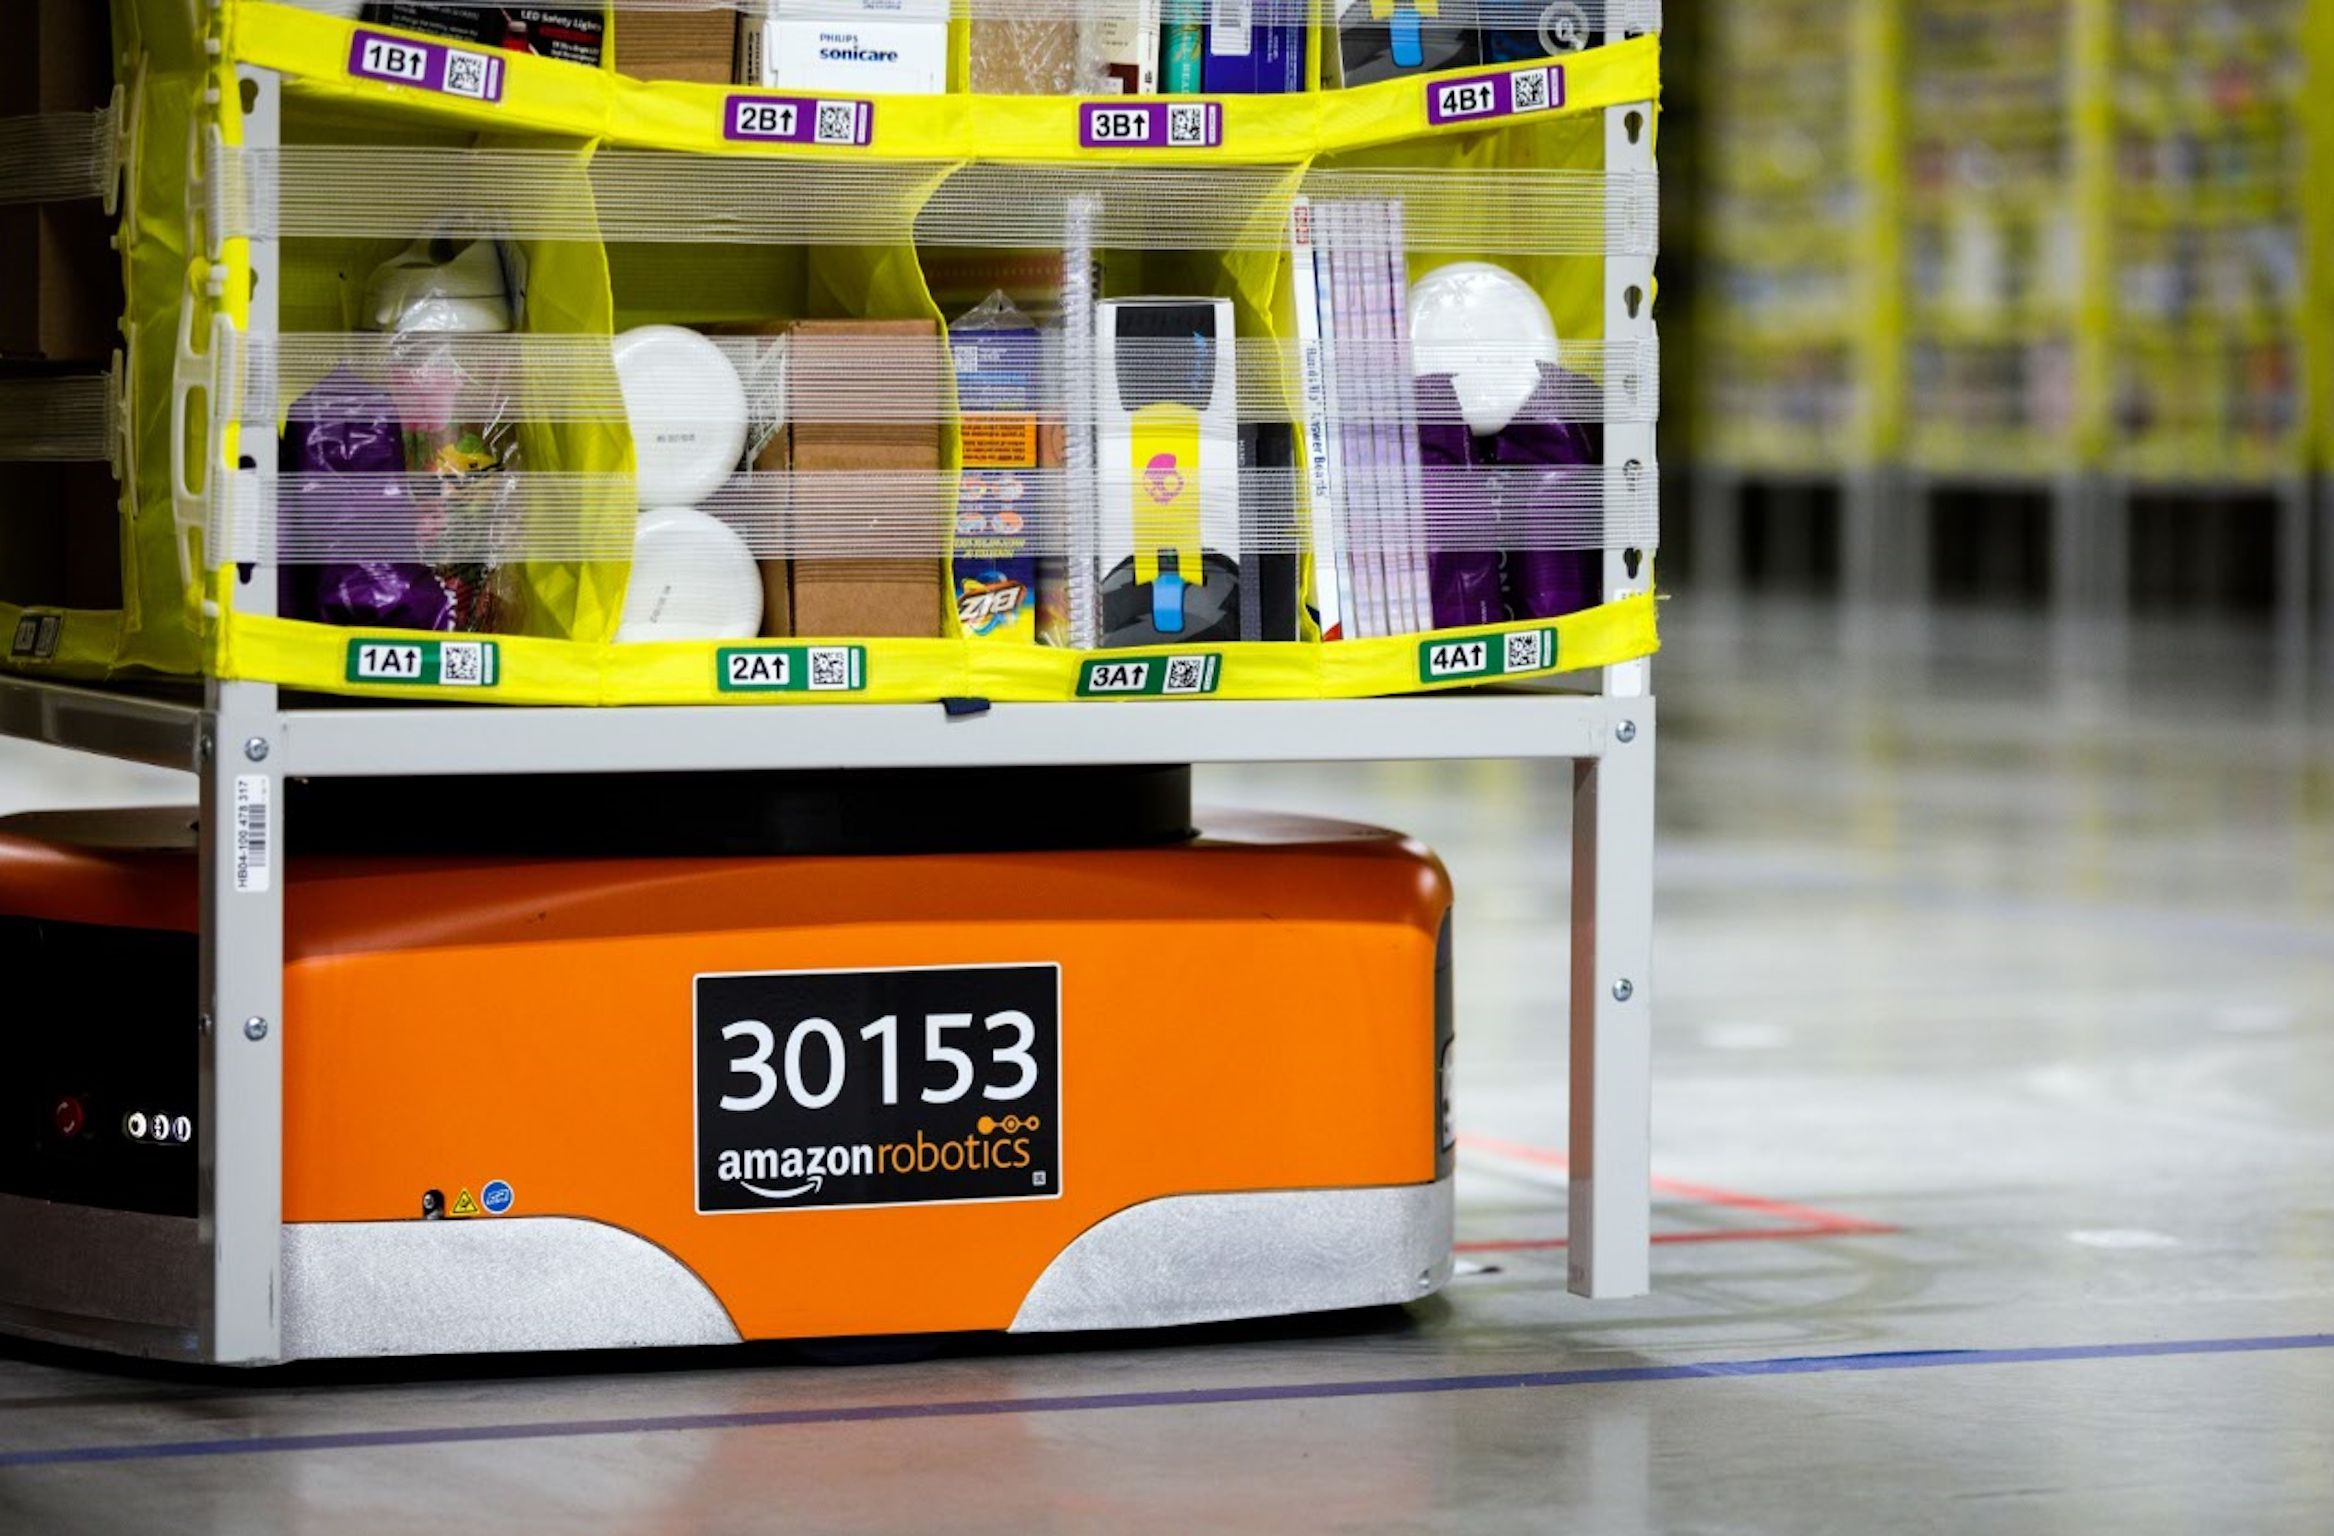
\includegraphics[width=0.6\linewidth]{figures/Amazon_Warehouse.jpeg}
    \caption{Kiva system operating in Amazon warehouse.\protect\footnotemark}
    \label{fig:Amazon Warehouse Robots}
\end{figure}

\footnotetext{https://spectrum.ieee.org/interview-brad-porter-vp-of-robotics-at-amazon}


\begin{itemize}
    \item \textbf{Warehouse Automation}: Automated pick-pack-and-ship system in warehouse (like Fig \ref{fig:Amazon Warehouse Robots}.) \cite{Amazon_Kiva}. Delivering items in sorting station\cite{Warehouse_Automation1,Warehouse_Automation2}.
    \item \textbf{Intersection Management}: Coordinate autonomous vehicle movement through intersections \cite{Intersection_Management}.
    \item \textbf{Robot Fleet}: Automating fleets of autonomous robots like forklift fleets \cite{Fork_Fleet1,Fork_Fleet2}.  
    \item \textbf{Agents in video games and CGIs}: Flock simulating and animating\cite{Flocking_1,Flocking_2}.
    \item \textbf{Swarm Robots}: Controlling self-organised robot swarms\cite{Swarm_Robotics}.
\end{itemize}

In general, the application of this algorithm is very broad. Furthermore, in the context of Industry 4.0 and flexible manufacturing, it has even better prospects for application\cite{Industry_41,Industry_42,Industry_43}, as centralized control is gradually becoming inadequate to meet new production needs.
